\documentclass{article}
\usepackage[utf8]{inputenc}
\usepackage{amssymb}
\usepackage{amsfonts}
\usepackage{amsmath}
\usepackage[utf8]{inputenc}
\usepackage[english]{babel}
\usepackage{lmodern}
\usepackage{float}
\usepackage{graphicx}
\DeclareGraphicsExtensions{.eps,.pdf,.png,.jpg}
\usepackage{latexsym}
\usepackage{hyperref}
\usepackage[euler]{textgreek}
\usepackage{stackengine}
\usepackage{listings}
\usepackage[version-1-compatibility]{siunitx}
\usepackage[usenames,dvipsnames]{xcolor}
\usepackage{pdfpages}
\hypersetup{pdfborder={0 0 0}}
\usepackage{pgfplots}
\pgfplotsset{compat=newest}
\pgfplotsset{plot coordinates/math parser=false}
\newlength\figureheight
\newlength\figurewidth
\usepackage[section]{placeins}%Sørger for at plots og andre floats holder seg til sin section.

\definecolor{dkgreen}{rgb}{0,0.6,0}
\definecolor{gray}{rgb}{0.5,0.5,0.5}
\definecolor{pink}{rgb}{0.63, 0.13, 0.94}
\lstset{language=Matlab, 
    keywords={break, case, catch, continue,else,elseif,end,for,function,
        global,if,otherwise,persistent,return,switch,try,while},
    basicstyle=\ttfamily,
    keywordstyle=\color{blue},
    commentstyle=\color{dkgreen},
    stringstyle=\color{pink},
    numbers=left,
    numberstyle=\tiny\color{gray},
    stepnumber=1,
    numbersep=10pt,
    backgroundcolor=\color{white},
    tabsize=4,
    showspaces=false,
    showstringspaces=false}


\title{Exercise 7 - TTK4130 Modeling and Simulation}
\author{Camilla Sterud}
\date{}

\begin{document}

\maketitle

\newpage

\section{Problem 1}

\begin{align*}
    \frac{\partial p(x,t)}{\partial t} &= -c Z_0 \frac{\partial q(x,t)}{\partial x}\\
    \frac{\partial q(x,t)}{\partial t} &= -\frac{c}{Z_0} \frac{\partial p(x,t)}{\partial x} - \frac{F(q(x,t))}{\rho_0}\\
    c &= \sqrt{\frac{\beta}{\rho_0}}\\
    Z_0 &= \frac{\rho_0 c}{A} = \frac{\sqrt{\rho_0\beta}}{A}\\
    F &= \rho_0Bq\\
    B &= \frac{8\nu_0}{r_0^2} 
\end{align*}

Helmholtz mass balance 
\begin{equation}\label{eq:massbal}
    \frac{V}{\beta} \dot p = q
\end{equation}

Helmholtz moment balance 
\begin{equation}\label{eq:momentbal}
    h\rho_0\dot q = -Ap
\end{equation}

\subsection{a}

Using Equation \ref{eq:massbal}, the mass balance for each volume can be set up as

\begin{equation*}
    \frac{V}{\beta}\dot p_i = q_{i-1} - q_i \Rightarrow \underline{\underline{\dot p_i = \frac{c^2\rho_0}{Ah}(q_{i-1} - q_i)}}.
\end{equation*}

Using Equation \ref{eq:momentbal}, the moment balance for each volume can be set up as


\begin{equation*}
    h\rho_0\dot q_i = -A(p_{i-1} - p_i) - Fh \Rightarrow \underline{\underline{\dot q_{i-1} = \frac{A}{h\rho_0}(p_{i-1} - p_i) - Bq_{i-1}}}.
\end{equation*}

\subsection{b}

\begin{align*}
    \dot{\mathbf{x}} &= \mathbf{Ax} + \mathbf{Bu}\\
    \mathbf{y} &= \mathbf{Cx} + \mathbf{Du}\\
    \mathbf{u} &= \begin{bmatrix}
        q_0\\q_N
    \end{bmatrix} \text{ and } 
    \mathbf{y} = \begin{bmatrix}
        p_1\\p_N
    \end{bmatrix}\\
    \mathbf{x}^T &= \begin{bmatrix}
        p_1 & q_1 & p_2 & q_2 & ... & q_{N-1} & p_N
    \end{bmatrix}
\end{align*}


\begin{equation*}
    \mathbf{A} = \begin{bmatrix}
        0 & -\frac{c^2\rho_0}{Ah} & 0 & \hdotsfor{4} & 0\\
        \frac{A}{h\rho_0} & -B & -\frac{A}{h\rho_0} & 0 & \hdotsfor{3} & 0\\
        0 & \frac{c^2\rho_0}{Ah} & 0 & -\frac{c^2\rho_0}{Ah} &  0 & \hdotsfor{2} & 0\\
        0 & 0 & \frac{A}{h\rho_0} & -B & -\frac{A}{h\rho_0} & 0 & \hdots & 0\\
        \vdots & \vdots & \ddots & \ddots & \ddots & \ddots & \ddots & \vdots \\
        0 & 0 &  \hdotsfor{1} & 0 & \frac{c^2\rho_0}{Ah} & 0 & -\frac{c^2\rho_0}{Ah}& 0\\
        0 & 0 & \hdotsfor{2} & 0 & \frac{A}{h\rho_0} & -B & -\frac{A}{h\rho_0}\\
        0 & 0 & \hdotsfor{3} & 0 & \frac{c^2\rho_0}{Ah}& 0
    \end{bmatrix}
\end{equation*}

\begin{align*}
    \mathbf{B} &= \begin{bmatrix}
        \frac{c^2\rho_0}{Ah} & 0\\
        0 & \vdots\\
        \vdots & \vdots\\
        \vdots & 0 \\
        0 & -\frac{c^2\rho_0}{Ah}
    \end{bmatrix}\\
    \mathbf{C} &= \begin{bmatrix}
        1 & 0 & \hdots & \hdots & 0\\
        0 & \hdots & \hdots & 0 & 1
    \end{bmatrix}\\
    \mathbf{D} &= 0
\end{align*}

The diagonal and the 1st and -1st superdiagonal of A alternate between two values. This makes it easy to implement in MATLAB. 

\subsection{d}

The response is quite similar for the three values of $N$, as seen in Figure \ref{fig:1c}. When consulting the bode plots in figures \ref{fig:1c_bode_p1} and \ref{fig:1c_bode_pN}, it is clear that the system is more oscillating for large values of $N$.
The code for generating these plots can be seen in listings \ref{lst:init} and \ref{lst:plot}

\begin{figure}[H]
    \centering
    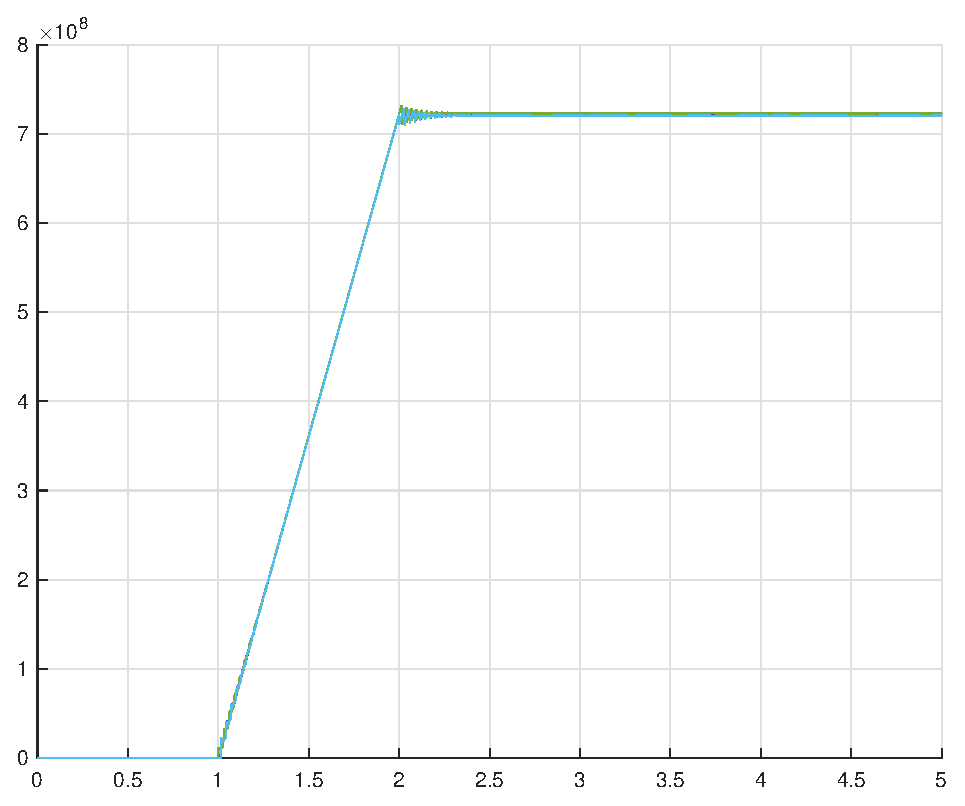
\includegraphics[width = 0.8\textwidth]{ex7_1c}
    \caption{$p_1$ and $p_N$ plotted for all values of $N$.}
    \label{fig:1c}
\end{figure}

\begin{figure}[H]
    \centering
    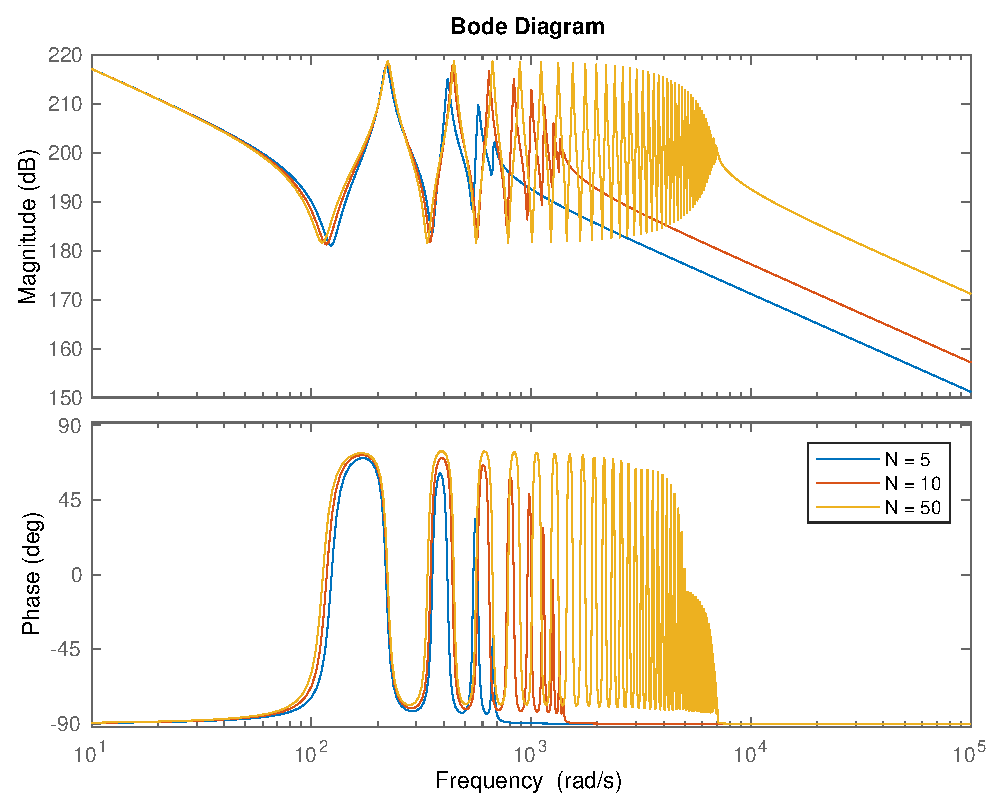
\includegraphics[width = 0.8\textwidth]{ex7_1c_bode_p1}
    \caption{Bode plot of the response from $q_0$ to $p_1$ for all values of $N$.}
    \label{fig:1c_bode_p1}
\end{figure}

\begin{figure}[H]
    \centering
    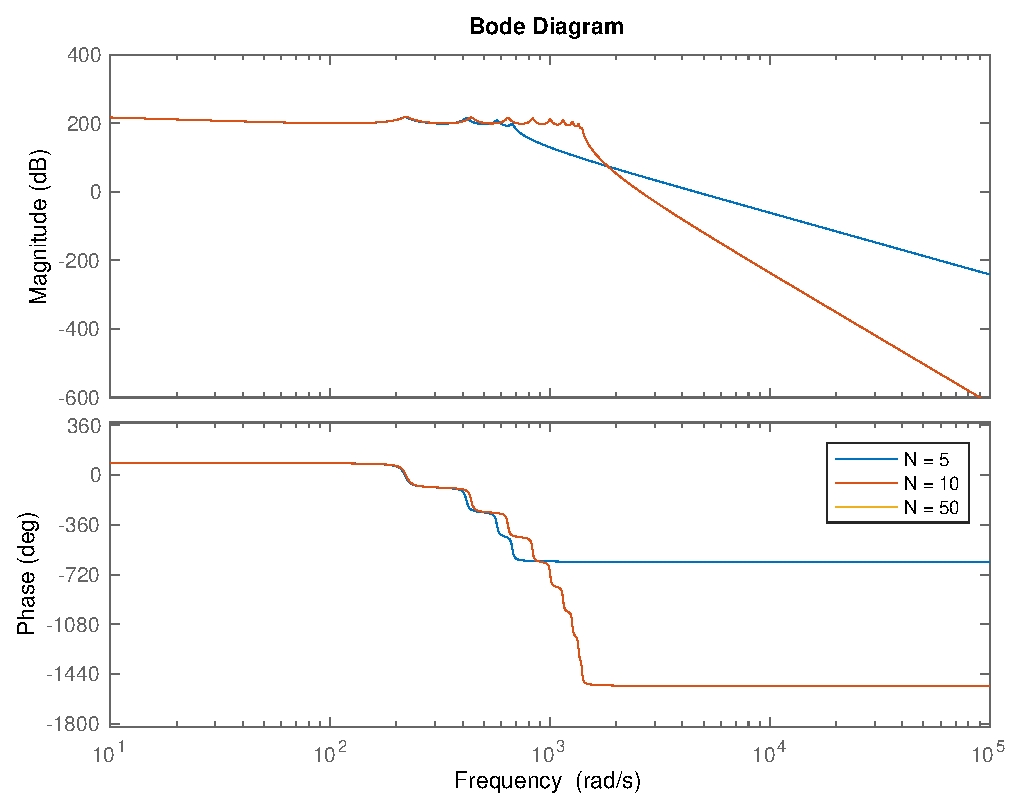
\includegraphics[width = 0.8\textwidth]{ex7_1c_bode_pN}
    \caption{Bode plot of the response from $q_0$ to $p_N$ for all values of $N$.}
    \label{fig:1c_bode_pN}
\end{figure}

\section{Problem 2}

\begin{equation}\label{eq:linfricdiff}
    \frac{\partial q}{\partial t} = -\frac{A}{\rho_0} \frac{\partial p}{\partial x} + \nu_0(\frac{\partial^2 q}{\partial x^2} - \frac{8}{r_0^2}q).
\end{equation}

\subsection{a}

Using that $\frac{\partial q_i}{\partial x} \simeq \frac{1}{h}(q_i - q_{i-1})$ for small $h$, twice, yields

\begin{equation*}
    \frac{\partial^2 q_i}{\partial x^2} \simeq \frac{1}{h}(\frac{\partial q_i}{\partial x} - \frac{\partial q_{i-1}}{\partial x}) \simeq \frac{1}{h}(\frac{1}{h}(q_i - q_{i-1}) - \frac{1}{h}(q_{i-1} - q_{i-2}))
\end{equation*}

\begin{equation*}
    \underline{\underline{\frac{\partial^2 q_i}{\partial x^2} = \frac{q_{i-2} - 2q_i + q_i}{h^2}}}
\end{equation*}

\subsection{b}

Discretizing in a similar manner as in Problem 1 

\begin{equation*}
    \underline{\underline{\dot p_i = \frac{c^2\rho_0}{Ah}(q_{i-1} - q_i)}}
\end{equation*}

\begin{equation*}
    q_{i-1} = -\frac{A}{h\rho_0}(p_{i} - p_{i-1}) + \nu_0(\frac{\partial^2 q_{i}}{\partial x^2} - \frac{8}{r_0^2}q_{i-1})
\end{equation*}

\begin{equation*}
    \underline{\underline{q_{i-1} = \frac{A}{h\rho_0}(p_{i-1} - p_{i}) - (\frac{2\nu_0}{h^2} + \frac{8}{r_0^2})q_{i-1} + \frac{\nu_0}{h^2}(q_{i-2} + q_i)}}
\end{equation*}


\begin{equation*}
    \mathbf{A} = \begin{bmatrix}
        0 & -\frac{c^2\rho_0}{Ah} & 0 & \hdotsfor{4} & 0\\
        \frac{A}{h\rho_0} & -(\frac{2\nu_0}{h^2} + \frac{8}{r_0^2}) & -\frac{A}{h\rho_0} & \frac{\nu_0}{h^2} & 0 & \hdotsfor{2} & 0\\
        0 & \frac{c^2\rho_0}{Ah} & 0 & -\frac{c^2\rho_0}{Ah} &  0 & \hdotsfor{2} & 0\\
        0 & \frac{\nu_0}{h^2} & \frac{A}{h\rho_0} & -(\frac{2\nu_0}{h^2} + \frac{8}{r_0^2}) & -\frac{A}{h\rho_0} & \frac{\nu_0}{h^2} & \hdots & 0\\
        \vdots & \vdots & \ddots & \ddots & \ddots & \ddots & \ddots & \vdots \\
        0 & 0 &  \hdotsfor{1} & 0 & \frac{c^2\rho_0}{Ah} & 0 & -\frac{c^2\rho_0}{Ah}& 0\\
        0 & 0 & \hdotsfor{1} & 0 & \frac{\nu_0}{h^2} & \frac{A}{h\rho_0} & -(\frac{2\nu_0}{h^2} + \frac{8}{r_0^2}) & -\frac{A}{h\rho_0}\\
        0 & 0 & \hdotsfor{3} & 0 & \frac{c^2\rho_0}{Ah}& 0
    \end{bmatrix}
\end{equation*}

\begin{align*}
    \mathbf{B} &= \begin{bmatrix}
        \frac{c^2\rho_0}{Ah} & 0\\
        \frac{\nu_0}{h^2} & 0\\
        0 & 0\\
        \vdots & \vdots \\
        0 & 0 \\
        0 & \frac{\nu_0}{h^2}\\
        0 & -\frac{c^2\rho_0}{Ah}
    \end{bmatrix}\\
    \mathbf{C} &= \begin{bmatrix}
        1 & 0 & \hdots & \hdots & 0\\
        0 & \hdots & \hdots & 0 & 1
    \end{bmatrix}\\
    \mathbf{D} &= 0
\end{align*}


\section{Problem 3}

\subsection{a}

Since $x_1$ and $x_2$ appear as time derivatives in the DAE, they are differential variables. $x_3$ is an algebraic variable, as its derivative does not appear. 

\subsection{b}

$x_1$ is dependent on $x_3$ (or the other way around), and $x_2$ s dependent on $x_1$. This means that there is only one independent variable in the system, and therefore the system has 1 degree of freedom. 

\subsection{c}

To transform the DAE to an ODE we have to differentiate twice:

\begin{align*}
    \frac{d}{dt}(x_1 - u) &= \dot x_1 -\dot u\\
    x_3 &= \dot u \\
    \frac{d^2}{dt^2}(x_1 - u) &= \dot x_3 - \ddot u\\
    \dot x_3 &= \ddot u
\end{align*}

Therefore, the system is of index 2. 

\subsection{d}

\begin{align*}
    0 &= x_3 - \dot u\\
    \dot x_2 &= x_1\\
    0 &= x_1 - u
\end{align*}


\lstinputlisting[label=lst:init,caption=Code for initialising a system with $N$ volumes., frame = single]{ModSim_ex7_1c_init.m}


\lstinputlisting[label=lst:plot,caption=Code for running and plotting a system with $N$ volumes., frame = single]{ModSim_ex7_1c.m}



\end{document}